%!TEX root=../Benutzerhandbuch.tex
\chapter{Installation}
\section{Start der Installation}
Die Installation wird durch das Ausf�hren der \inline{setup.exe} ge\-startet. Danach �ffnet sich der Installer.
\begin{figure}[!h]
\centering
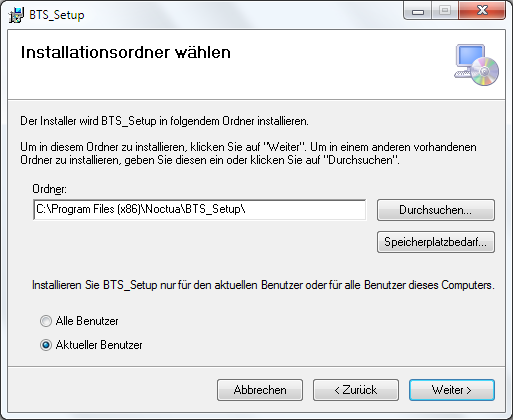
\includegraphics[width=1\textwidth]{images/btsinstall1.png}
\caption{Konfigurieren der Installation}
\end{figure}
Nach der korrekten Konfiguration des Setups kann die Installation gestartet werden.
\begin{figure}[!h]
\centering
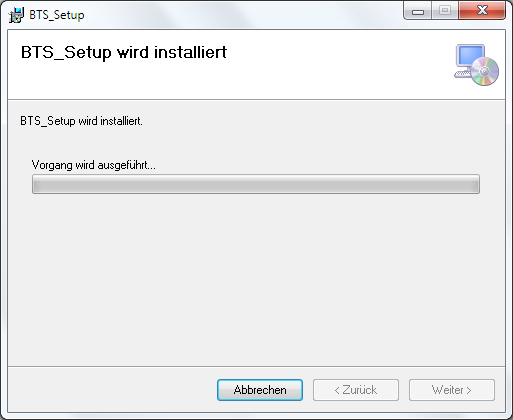
\includegraphics[width=1\textwidth]{images/btsinstall2.png}
\caption{Installationsvorgang}
\end{figure}
Nach diesem Vorgang ist die Backtesting-Software vollst�ndig installiert und ausf�hrbar.